\subsection*{RQ1: Scenarios and learning contexts}

In Figure \ref{fig:scenarios} the distribution of the encountered scenarios is presented. Most research is connected to schools and governance.
This is confirmed by the fact that the target population of the studies and/or the community affected by the learning process are often the students.

Several publications present a scenario where students are involved in the development of an architectural or urban planning project in the city, e.g. \cite{seitamaa-hakkarainen_architecture_2012},\cite{ulrich_lets_2013},\cite{beckett_augmented_2005}.

\begin{figure}[htb]
\centering
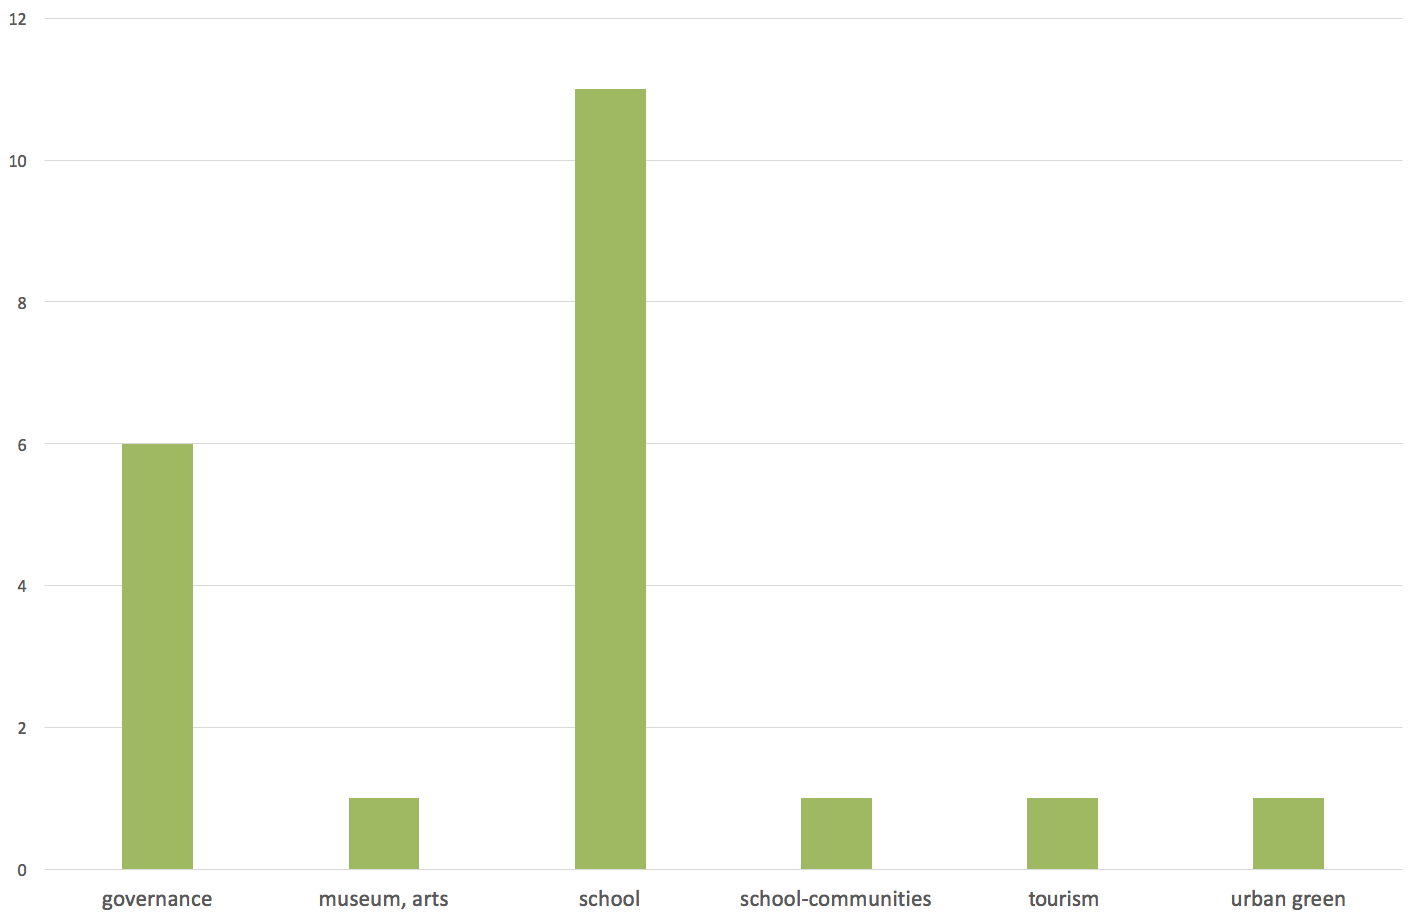
\includegraphics[width=12cm]{img/scenario}
\caption{Identified research scenarios.}
\label{fig:scenarios}
\end{figure}

This result can be correlated to the finding that more than 68\% of the articles present the concept of the city as a place where the learning experience happens. This point of view is quite distinct to the more engaging concept of actively living the city, learning behaviours and generating knowledge, which can be considered a lifelong learning experience to improve the quality of urban living.
As an example of this concept, some articles focus on promoting and teaching environmental-friendly practices like reducing the carbon footprint \cite{evans_give_2014} or reduce dependence on owned cars to satisfy mobility needs \cite{valle_cloud_2011}.


\subsection*{RQ2: Publication pattern}

Research on smart city learning gained approval and popularity quite constantly during the years. In Figure \ref{fig:years} the number of publications per year is showed. A relatively important amount of articles dates back to 2005, starting year of the chosen interval.

From 2006 a general increase in publications can be noted till 2014. The year 2015 was excluded from this statistic since not all research on the topic was yet published when articles were collected.

\begin{figure}[htb]
\centering
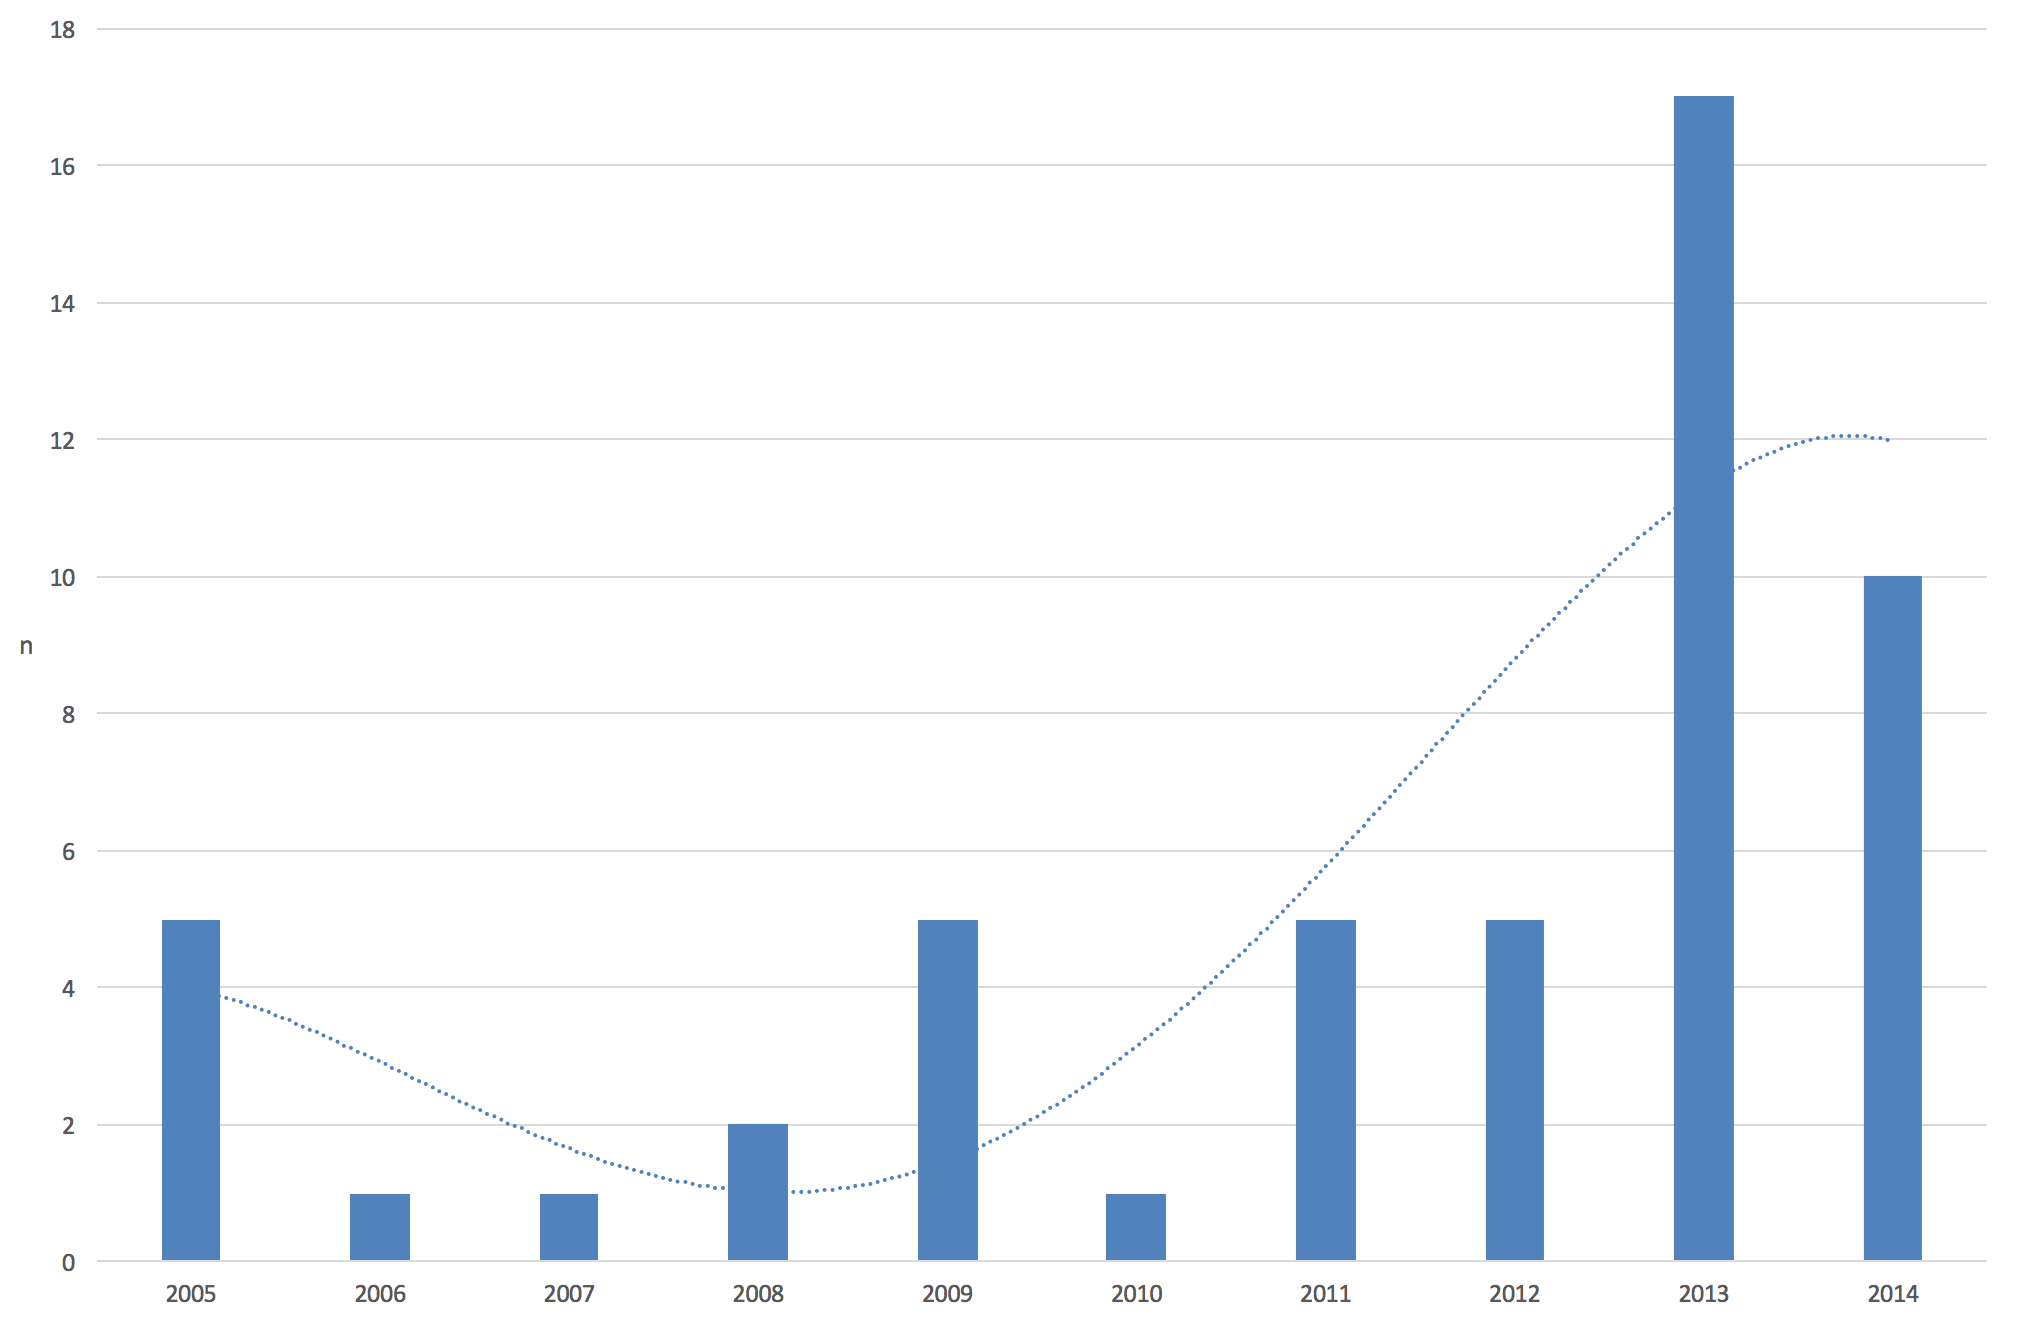
\includegraphics[width=12cm]{img/years}
\caption{Research publications per year. In dots: fourth order polynomial trendline.}
\label{fig:years}
\end{figure}

Selected articles are almost equally divided between international conference proceeding publications and journals or book chapters.
Publications from international journals is the most numerous category.


\subsection*{RQ3: Application of technology}

The technological pattern involved in smart city learning is, most of the times, connected to supporting the learning process, as visible in Figure \ref{fig:tech_patterns} where the frequency of the identified technological patterns is presented.
This means that technology is used as a tool to support a learning process that remains often structured as a traditional one.
Some of the others applications use technology to acquire and collect specific information like sensor data or geographical location.
From Figure \ref{fig:technology}, which gives an overview of technologies used, mobile devices emerge as the prevailing category.
As an example, studies adopt mobile technologies to generate and collect data \cite{philip_framework_2013},\cite{akkerman_storification_2009-1}, support language learning or others school topics and subjects \cite{gaved_challenges_2014} and as supporting technology in situated games in the city \cite{akkerman_storification_2009-1},\cite{huizenga_cognitive_2008}.

\begin{figure}[htb]
\centering
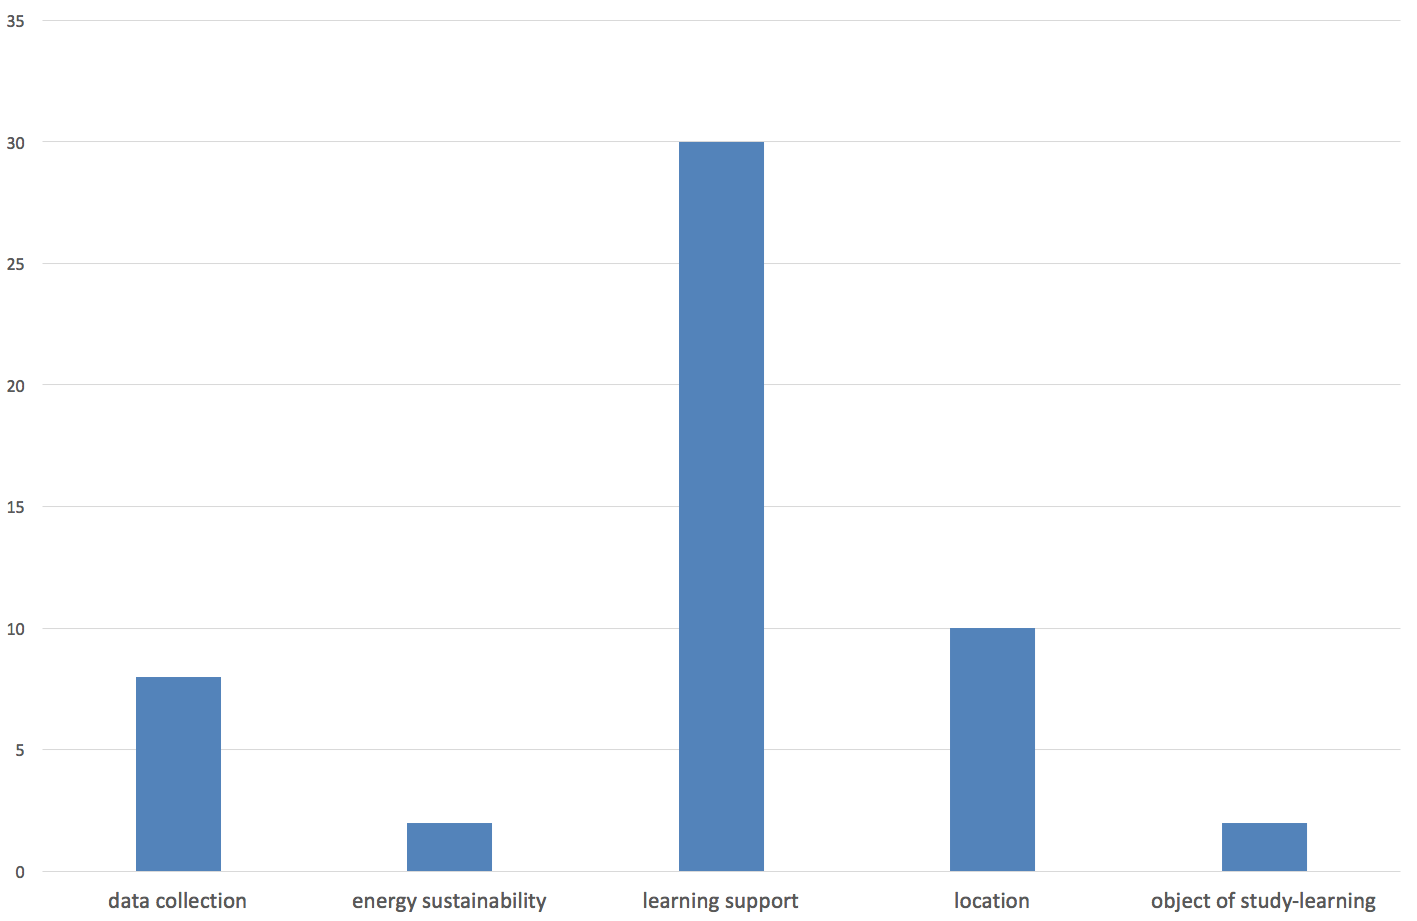
\includegraphics[width=12cm]{img/technological_pattern}
\caption{Identified technological patterns.}
\label{fig:tech_patterns}
\end{figure}

Online cooperative platforms of various types are also used in many cases: more precisely e-learning \cite{schneider_location_2007},\cite{kabaka_elearning_2013} and e-government solutions \cite{wong_prototype_2005},\cite{deakin_intelligent_2012} were mentioned in more than one article.

\begin{figure}[htb]
\centering
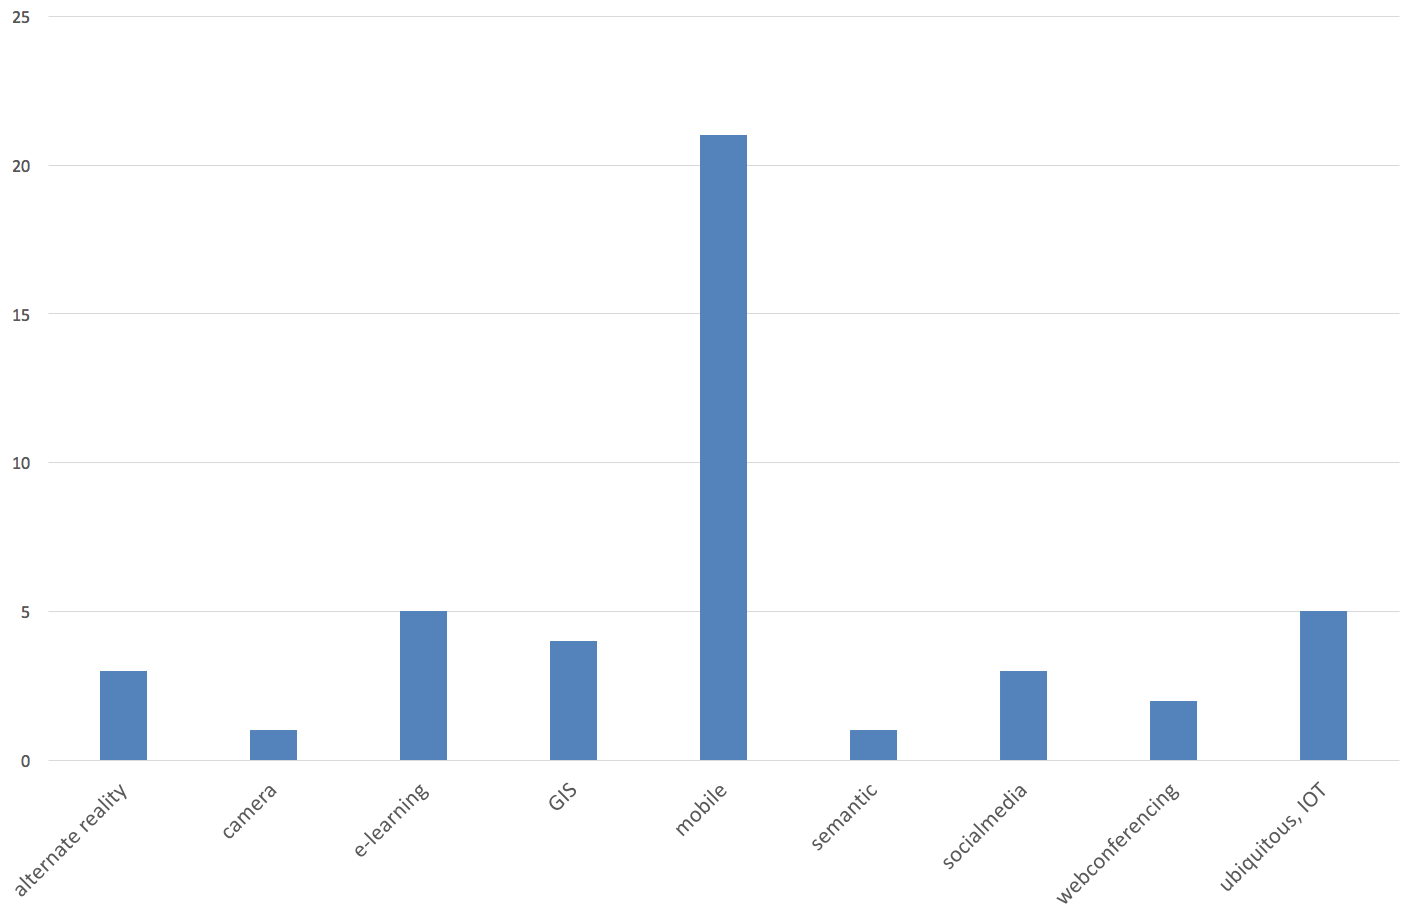
\includegraphics[width=12cm]{img/technology}
\caption{Technology use.}
\label{fig:technology}
\end{figure}


\subsection*{RQ4: Learning theories and approaches}

Some articles mentioned specific learning theories applied during the study. Game-based Learning and Situated Learning \cite{anderson_situated_1996} are the approaches that were reported more often.
Figure \ref{fig:learn_theories} pictures which learning theories are mentioned more often in the studies. It is also worth mentioning that most of the abstracts do not mention explicitly a specific learning theory.

The articles that use Game-Based Learning methods and serious games \cite{poplin_digital_2014-2}, often locate the gameplay in the urban space and make use of mobile devices \cite{huizenga_cognitive_2008}.

\begin{figure}[htb]
\centering
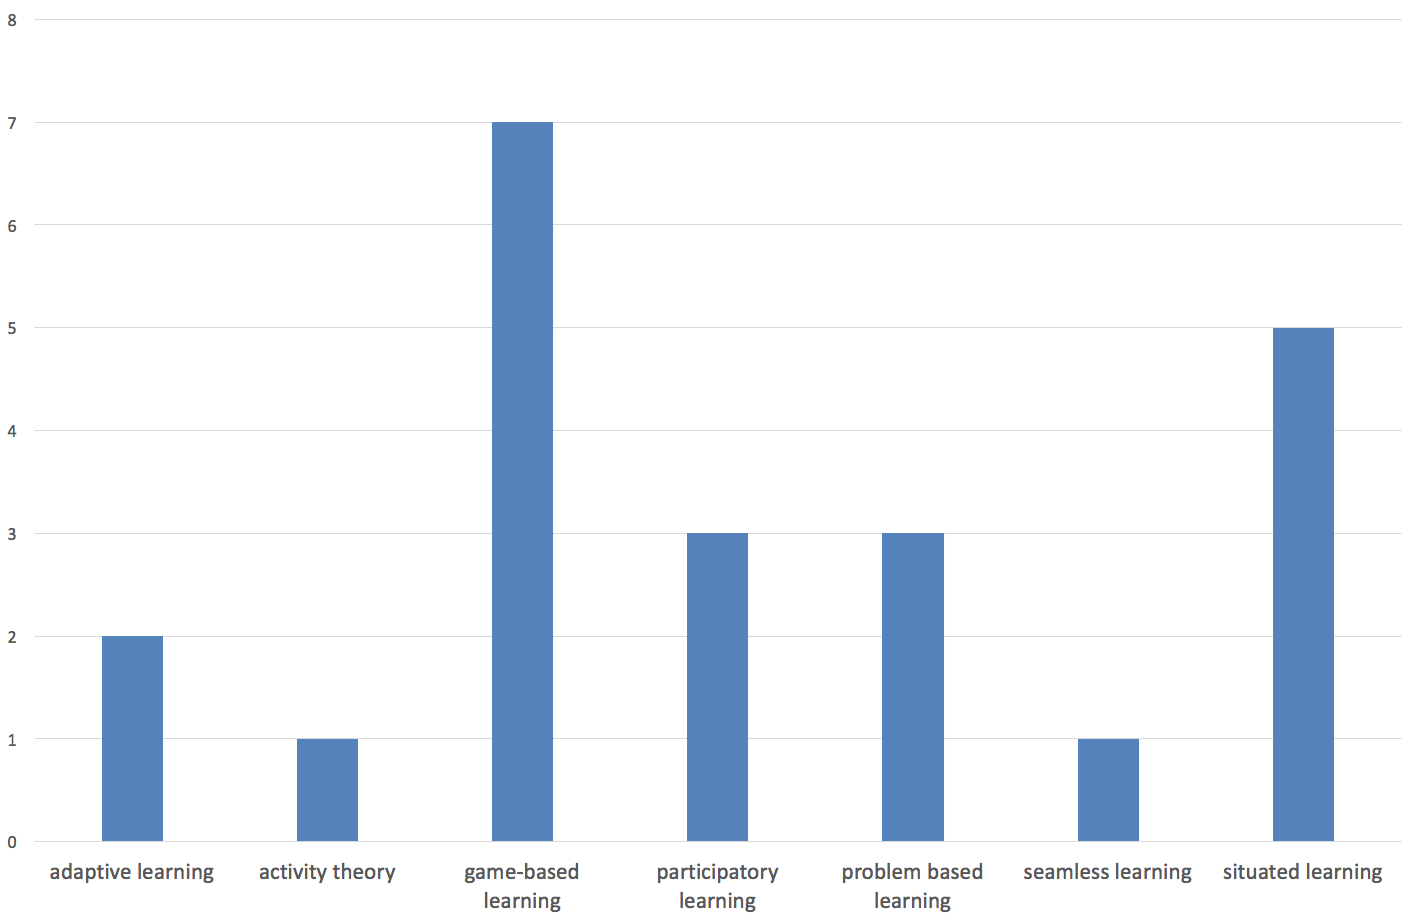
\includegraphics[width=12cm]{img/learning_theories}
\caption{Learning theories applied in the studies.}
\label{fig:learn_theories}
\end{figure}

Figure \ref{fig:approaches} describes some of the pursued approaches and concepts found in the abstracts screened.
The most referenced ones are connected to various levels of collaboration and cooperation between stakeholders or within the learning community (for example among the students). Context awareness and situatedness are also mentioned in a few articles.

Collaboration is crucial since many articles involve different stakeholders in the learning process, like universities and technical schools \cite{lee_platform_2011}, decision maker, citizens and universities \cite{evans_give_2014} or stakeholders located in different countries \cite{ross_facilitating_2009},\cite{severengiz_enhancing_2015}.

\begin{figure}[htb]
\centering
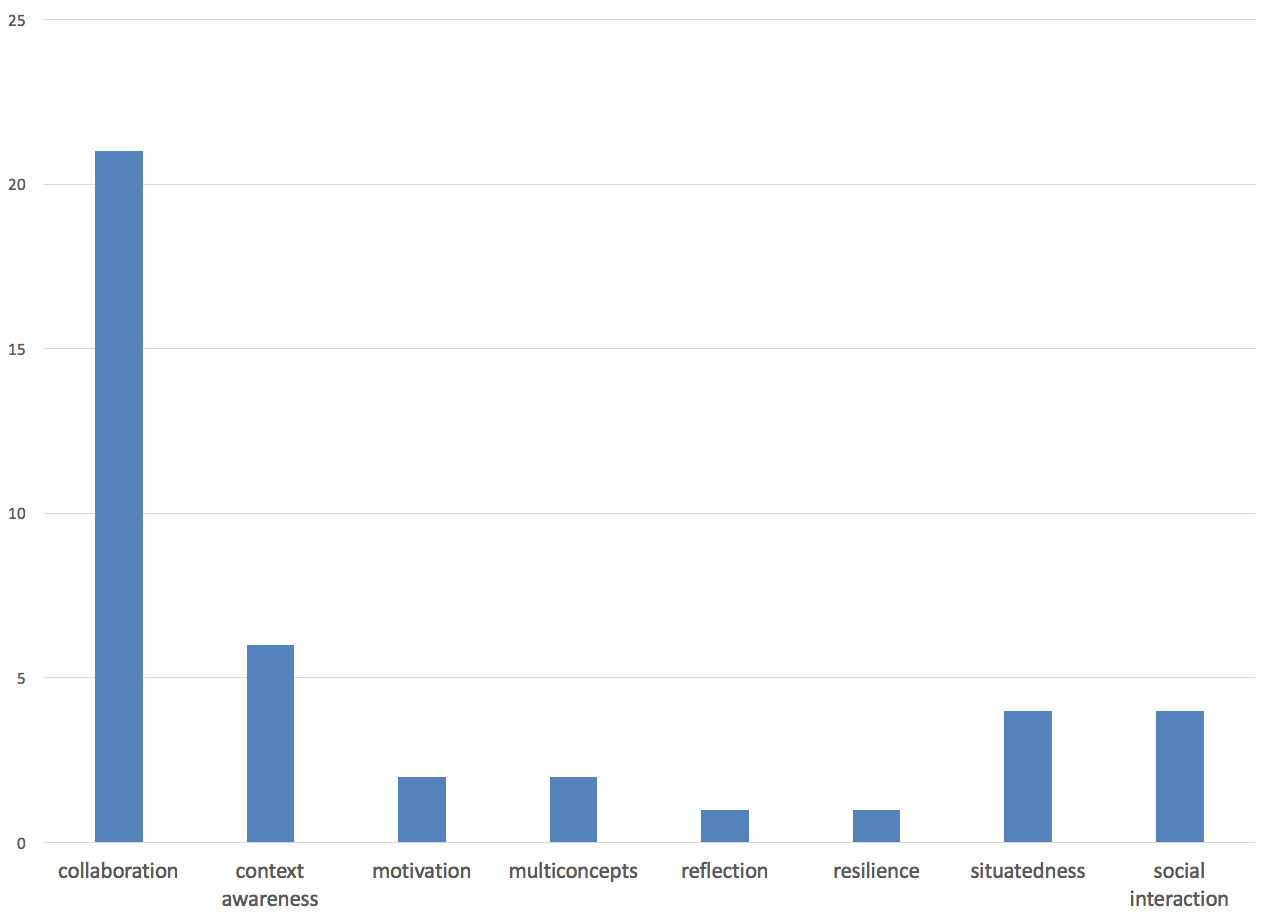
\includegraphics[width=12cm]{img/approaches}
\caption{Pursued approaches and concepts.}
\label{fig:approaches}
\end{figure}


\subsection*{RQ5: Research methods and types of research}
Research on smart city learning is often limited to perform a specific problem investigation.
Studies that aim to design a concrete solution or a technological implementation are less common.
This means that technology, although present, is not exploited for its full potential as a facilitator instrument but rather as a marginal supporting tool.

Even more rare are studies that make use of IOT, ubiquitous technologies and custom hardware prototyping.